\section{Resultat}
\label{sec:joel_a-results}
I denna del presenteras de resultat som framkom då metoden genomfördes, rent konkret så presenteras teamets koldioxidutsläpp till följd av utvecklingsprocessen samt användningen av molntjänster.s

\subsection{Utvecklingsprocessens koldioxidutsläpp}
Projektet var en del i en större universitetskurs som tog 400 timmar per teammedlem. Enligt teamets egna tidsrapportering så lades ungefär 30\% av dessa 400 timmar på utveckling. Vilken dator teamet utvecklade på varierade stort och för denna rapport så tillåts en av dessa datorer representera alla de andra. Teamet kunde se att programering på en dator av typ ’’Lenovo ideapad Y700’’ drog hela dess batteri ifrån 100\% till noll på ungefär fyra timmar. Enligt dess tillverkade Lenovo~\cite{lenovo} så har denna datormodell ett batteri med 60 watt timmar. En urladdning av detta på fyra timmar ger oss en timmes användning av 15 watt. Kombinerat med den uppskattade tiden fås följande ekvation fram: $$ 400 * 0.3 * 8* 15 = 14.4 \text{kW}$$

Enligt statistik ifrån Naturvårdsverket som kan ses i figur \ref{natuvard-co2} så skapade Sveriges el och värmeproduktion ett koldioxidutsläpp på $4781*10^9$ gram år 2016~\cite{naturvardsverket}. Kombinerat med att Sveriges energiproduktion detta år var 152 TWh enligt Energimyndighetens pressmeddelande\cite{elprod2016}, så får vi att varje kWh i genomsnitt skapade ett utsläpp på: $$4781*10^9 / (152 * 10^{12}) \approx 31.45 * 10^{-3} \text{ gram \ce{CO2} per kWh}$$ 
Kombinerat med uppskattningen av hur mycket elektricitet utvecklarnas datorer drog så får vi följande approximerade utsläpp: $$14.4 * 31.45 * 10^{-3} \approx 0.453 \text{ gram \ce{CO2}}$$

\begin{figure*}[!htbp]
	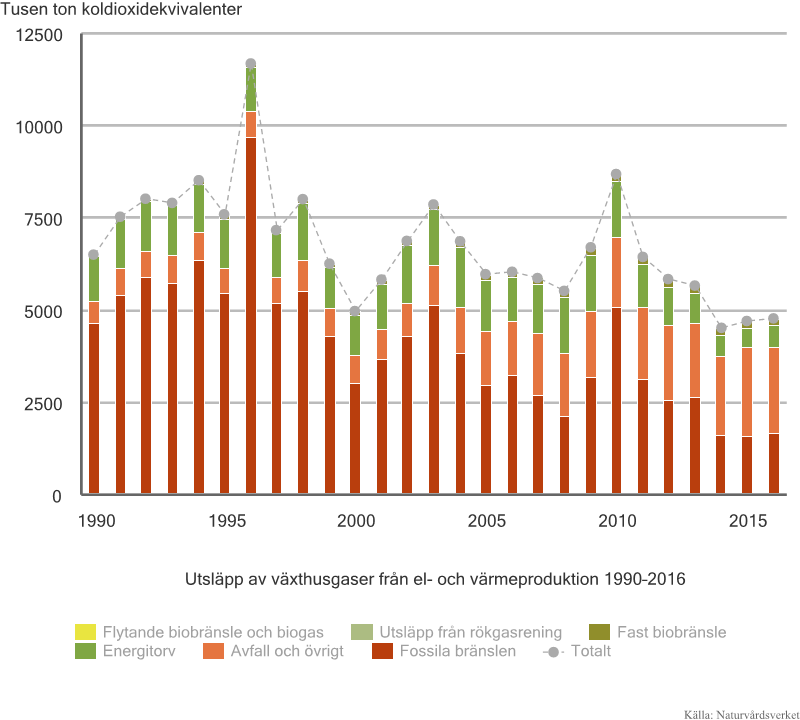
\includegraphics[scale=0.7]{naturvard-co2}
	\caption[Statistik ifrån naturvårdsverket gällande utsläpp av växthusgaser]{Statistik ifrån naturvårdsverket~\cite{naturvardsverket}}
	\label{natuvard-co2}
\end{figure*}



\subsection{Molntjänsternas koldioxidutsläpp}
En sammanställning av operationer teamet utförde mot Google Drive och Github ges i tabell \ref{tab:drive_results_table} och \ref{tab:github_results_table}. Operation i tabell \ref{tab:drive_results_table} syftar till hur ett objekt modifieras och de kategorier som finns är de namn som Google givit operationerna.

I avsnitt \ref{joel_a-method-cloud-eq} så togs en approximation fram för hur mycket koldioxid som generas vid varje operation. Multiplicerar vi denna med antalet operationer så får vi ut hur mycket koldioxid användning av molntjänster skapad. $$(577 + 136) * 0.6 = 427.8 \text{ gram \ce{CO2}}$$

\begin{table}[H]
	\centering
	\begin{tabular}{| l | l |}
		\cline{1-2}
		\multicolumn{1}{| c |}{\textbf{Operation}} & \textbf{Antal}  \\ \hline
		Redigera & 262 \\ \hline
		Kopiera & 43 \\ \hline
		Kommentera & 4 \\ \hline
		Byta namn & 40 \\ \hline
		Ladda upp & 95 \\ \hline
		Skapa & 92 \\ \hline
		Flytta & 39 \\ \hline
		Ta bort & 2 \\ \hline
		\textbf{Totalt} & \textbf{577}\\ \hline
	\end{tabular}
	\caption{Antal operationer teamet gjort på Google drive}
	\label{tab:drive_results_table}
\end{table}

\begin{table}[H]
	\centering
	\begin{tabular}{| l | l |}
		\cline{1-2}
		\multicolumn{1}{| c |}{\textbf{Gitrepo}} & \textbf{Antal push operationer}\\ \hline
		UI & 31 \\ \hline
		Kontroller & 26 \\ \hline
		Services & 12 \\ \hline
		Dokument & 67 \\ \hline
		Server & 0 \\ \hline
		\textbf{Totalt} & \textbf{136} \\ \hline
	\end{tabular}
	\caption{Antal git push operationer som gruppen gjort mot huvudgrenen på Githubs hemsida}
	\label{tab:github_results_table}
\end{table}







